\documentclass[border=4pt,varwidth=6in]{standalone}
\usepackage[T1]{fontenc}
\usepackage{mathptmx}
\usepackage[scaled=0.92]{helvet}
\usepackage{courier}
\usepackage{setspace}
\usepackage{amsmath,amssymb,amsthm}
\usepackage{xcolor}
\usepackage{graphicx}
\usepackage{float}
\usepackage[font={singlespacing,normalsize},labelfont=bf,labelsep=period,justification=justified,singlelinecheck=false]{caption}
\usepackage{subcaption}
\usepackage{booktabs,multirow,longtable,threeparttable,array,tabularx}
\usepackage{enumitem}
%% preamble.tex — packages and macros shared by all chapters
% Engine compatibility: biber writes UTF-8 into the .bbl. Under pdfTeX, inputenc maps
% characters outside Latin-1 to T1 glyphs; under XeTeX (tectonic) they would be silently
% dropped from the 8-bit Times fonts, so map them explicitly.
\usepackage{iftex}
\ifXeTeX
  \usepackage{newunicodechar}
  \newunicodechar{č}{\v{c}}\newunicodechar{Č}{\v{C}}\newunicodechar{ě}{\v{e}}\newunicodechar{ř}{\v{r}}
  \newunicodechar{š}{\v{s}}\newunicodechar{Š}{\v{S}}\newunicodechar{ž}{\v{z}}\newunicodechar{Ž}{\v{Z}}
  \newunicodechar{Ł}{\L{}}\newunicodechar{ł}{\l{}}\newunicodechar{ń}{\'n}\newunicodechar{ś}{\'s}
  \newunicodechar{ć}{\'c}\newunicodechar{ż}{\.z}\newunicodechar{ź}{\'z}\newunicodechar{ę}{\k{e}}\newunicodechar{ą}{\k{a}}
  \newunicodechar{ő}{\H{o}}\newunicodechar{ű}{\H{u}}\newunicodechar{ğ}{\u{g}}\newunicodechar{ş}{\c{s}}\newunicodechar{ı}{\i}
\fi
\usepackage{physics}          % \ket, \bra, \expval, \dd, \abs, \norm
\usepackage{bm}
\usepackage{mathtools}
\usepackage{siunitx}
\sisetup{detect-all,per-mode=symbol,range-phrase=--,range-units=single}
\usepackage{tikz}
\usetikzlibrary{quantikz2}
\usetikzlibrary{arrows.meta,positioning,calc,shapes.geometric,fit,backgrounds,matrix,decorations.pathreplacing}
\usepackage{pgfplots}
\pgfplotsset{compat=1.18}
\usepgfplotslibrary{groupplots,fillbetween}
\usepackage[ruled,vlined,linesnumbered]{algorithm2e}
\SetAlFnt{\singlespacing\small}
% cleveref is loaded by ttuthesis.cls *before* algorithm2e, so its algorithm2e alias is never
% installed; name the algocf label type explicitly so \cref{alg:...} prints "Algorithm N".
\usepackage{listings}
\lstset{basicstyle=\ttfamily\footnotesize\singlespacing,breaklines=true,columns=fullflexible,
        keepspaces=true,frame=single,framerule=0.3pt,xleftmargin=1em,showstringspaces=false,
        commentstyle=\itshape\color{black!60},keywordstyle=\bfseries}
\lstdefinelanguage{qasm}{morekeywords={OPENQASM,include,qubit,bit,h,cx,rz,ry,measure,reset,barrier},sensitive=true,morecomment=[l]{//}}

% Theorem-like environments (numbered per chapter, Arabic chapter number)

% Color-blind-safe palette for plots (also varies markers/line styles: TTU accessibility rule)
\definecolor{cbBlue}{HTML}{0072B2}
\definecolor{cbOrange}{HTML}{E69F00}
\definecolor{cbGreen}{HTML}{009E73}
\definecolor{cbRed}{HTML}{D55E00}
\definecolor{cbPurple}{HTML}{CC79A7}
\definecolor{cbSky}{HTML}{56B4E9}
\definecolor{cbGray}{HTML}{555555}
\pgfplotscreateplotcyclelist{ttu}{%
  {cbBlue,mark=*,solid},{cbOrange,mark=square*,dashed},{cbGreen,mark=triangle*,dotted},
  {cbRed,mark=diamond*,dashdotted},{cbPurple,mark=pentagon*,densely dashed},{cbGray,mark=o,loosely dotted}}
\pgfplotsset{every axis/.append style={cycle list name=ttu,width=0.8\linewidth,height=0.5\linewidth,
  tick label style={font=\small},label style={font=\small},legend style={font=\footnotesize,cells={anchor=west}},
  grid=major,grid style={black!12}}}

% Domain macros
\newcommand{\qgear}{Q-GEAR}
\newcommand{\deal}{DEAL}
\newcommand{\qawa}{QAWA}
\newcommand{\qpie}{QPIE}
\newcommand{\vqt}{VQT}
\newcommand{\shardq}{ShardQ}
\newcommand{\nnqa}{NNQA}
\newcommand{\rubriq}{RubriQ}
\newcommand{\cudaq}{CUDA-Q}
\newcommand{\qiskit}{Qiskit}
\newcommand{\qcrank}{QCrank}
\newcommand{\bigO}[1]{\mathcal{O}\!\left(#1\right)}
\newcommand{\Hcost}{H_C}
\newcommand{\Hmix}{H_M}
\newcommand{\code}[3]{[[#1,#2,#3]]}
\newcommand{\eps}{\varepsilon}
\newcommand{\R}{\mathbb{R}}
\newcommand{\C}{\mathbb{C}}
\newcommand{\Z}{\mathbb{Z}}
% \Tr provided by physics
\DeclareMathOperator{\poly}{poly}
\DeclareMathOperator*{\argmin}{arg\,min}
\DeclareMathOperator*{\argmax}{arg\,max}

\newcommand{\todo}[1]{{\color{red!70!black}\textbf{[TODO: #1]}}}
\providecommand{\cref}[1]{#1}
\providecommand{\Cref}[1]{#1}
\providecommand{\labelcref}[1]{#1}
\providecommand{\ref}[1]{#1}
\providecommand{\cite}[1]{[#1]}
\begin{document}
\begin{figure}[H]
\centering
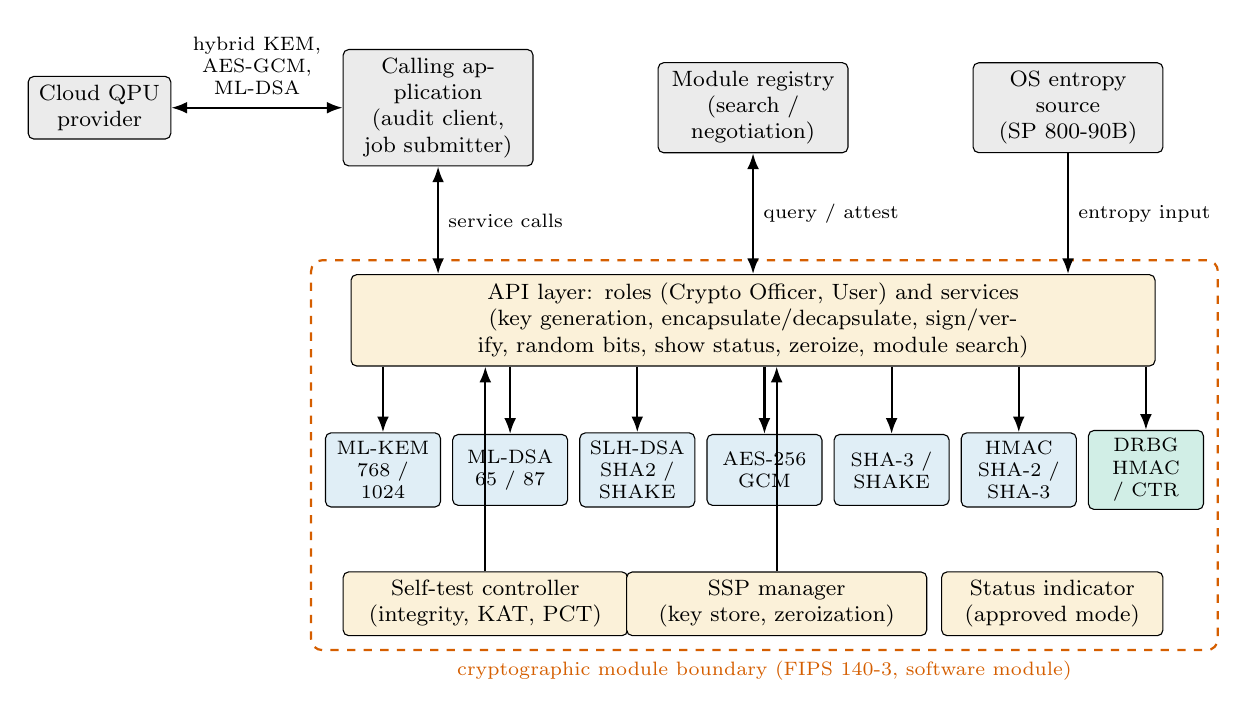
\begin{tikzpicture}[
  font=\footnotesize,
  blk/.style={draw,rounded corners=2pt,align=center,inner sep=3pt,minimum height=7mm},
  alg/.style={blk,fill=cbBlue!12,text width=12.5mm,minimum height=9mm,font=\scriptsize},
  ctl/.style={blk,fill=cbOrange!15},
  ext/.style={blk,fill=cbGray!12,text width=22mm},
  arr/.style={-{Latex[length=2mm]},thick},
  darr/.style={{Latex[length=2mm]}-{Latex[length=2mm]},thick}]
  \node[ctl,text width=100mm] (api) at (0,0) {API layer: roles (Crypto Officer, User) and services (key generation, encapsulate/decapsulate, sign/verify, random bits, show status, zeroize, module search)};
  \node[alg] (kem) at (-47mm,-19mm) {ML-KEM\\ 768 / 1024};
  \node[alg,right=1.4mm of kem] (dsa) {ML-DSA\\ 65 / 87};
  \node[alg,right=1.4mm of dsa] (slh) {SLH-DSA\\ SHA2 / SHAKE};
  \node[alg,right=1.4mm of slh] (aes) {AES-256\\ GCM};
  \node[alg,right=1.4mm of aes] (sha) {SHA-3 /\\ SHAKE};
  \node[alg,right=1.4mm of sha] (hmac) {HMAC\\ SHA-2 / SHA-3};
  \node[alg,right=1.4mm of hmac,fill=cbGreen!18] (drbg) {DRBG\\ HMAC / CTR};
  \node[ctl,text width=34mm] (st) at (-34mm,-36mm) {Self-test controller\\ (integrity, KAT, PCT)};
  \node[ctl,text width=36mm] (ssp) at (3mm,-36mm) {SSP manager\\ (key store, zeroization)};
  \node[ctl,text width=26mm] (ind) at (38mm,-36mm) {Status indicator\\ (approved mode)};
  \begin{scope}[on background layer]
    \node[draw,cbRed,dashed,thick,rounded corners=4pt,fit=(api)(kem)(drbg)(st)(ssp)(ind),inner sep=5pt,
          label={[cbRed,font=\scriptsize]below:cryptographic module boundary (FIPS 140-3, software module)}] (bd) {};
  \end{scope}
  \node[ext] (app) at (-40mm,27mm) {Calling application\\ (audit client, job submitter)};
  \node[ext] (reg) at (0,27mm) {Module registry\\ (search / negotiation)};
  \node[ext] (ent) at (40mm,27mm) {OS entropy source\\ (SP 800-90B)};
  \node[ext,text width=16mm] (cloud) at (-83mm,27mm) {Cloud QPU\\ provider};
  \draw[darr] (app.south) -- (app.south|-api.north) node[midway,right,font=\scriptsize]{service calls};
  \draw[darr] (reg.south) -- (reg.south|-api.north) node[midway,right,font=\scriptsize]{query / attest};
  \draw[arr] (ent.south) -- (ent.south|-api.north) node[midway,right,font=\scriptsize]{entropy input};
  \foreach \n in {kem,dsa,slh,aes,sha,hmac,drbg}{\draw[arr] (api.south -| \n) -- (\n.north);}
  \draw[arr] (st.north) -- (st.north|-api.south);
  \draw[arr] (ssp.north) -- (ssp.north|-api.south);
  \draw[darr] (app.west) -- (cloud.east) node[midway,above=1pt,font=\scriptsize,align=center]{hybrid KEM,\\ AES-GCM,\\ ML-DSA};
\end{tikzpicture}
\end{figure}
\end{document}
